\documentclass{standalone}
\usepackage{tikz}
\usetikzlibrary{patterns, positioning}

\begin{document}
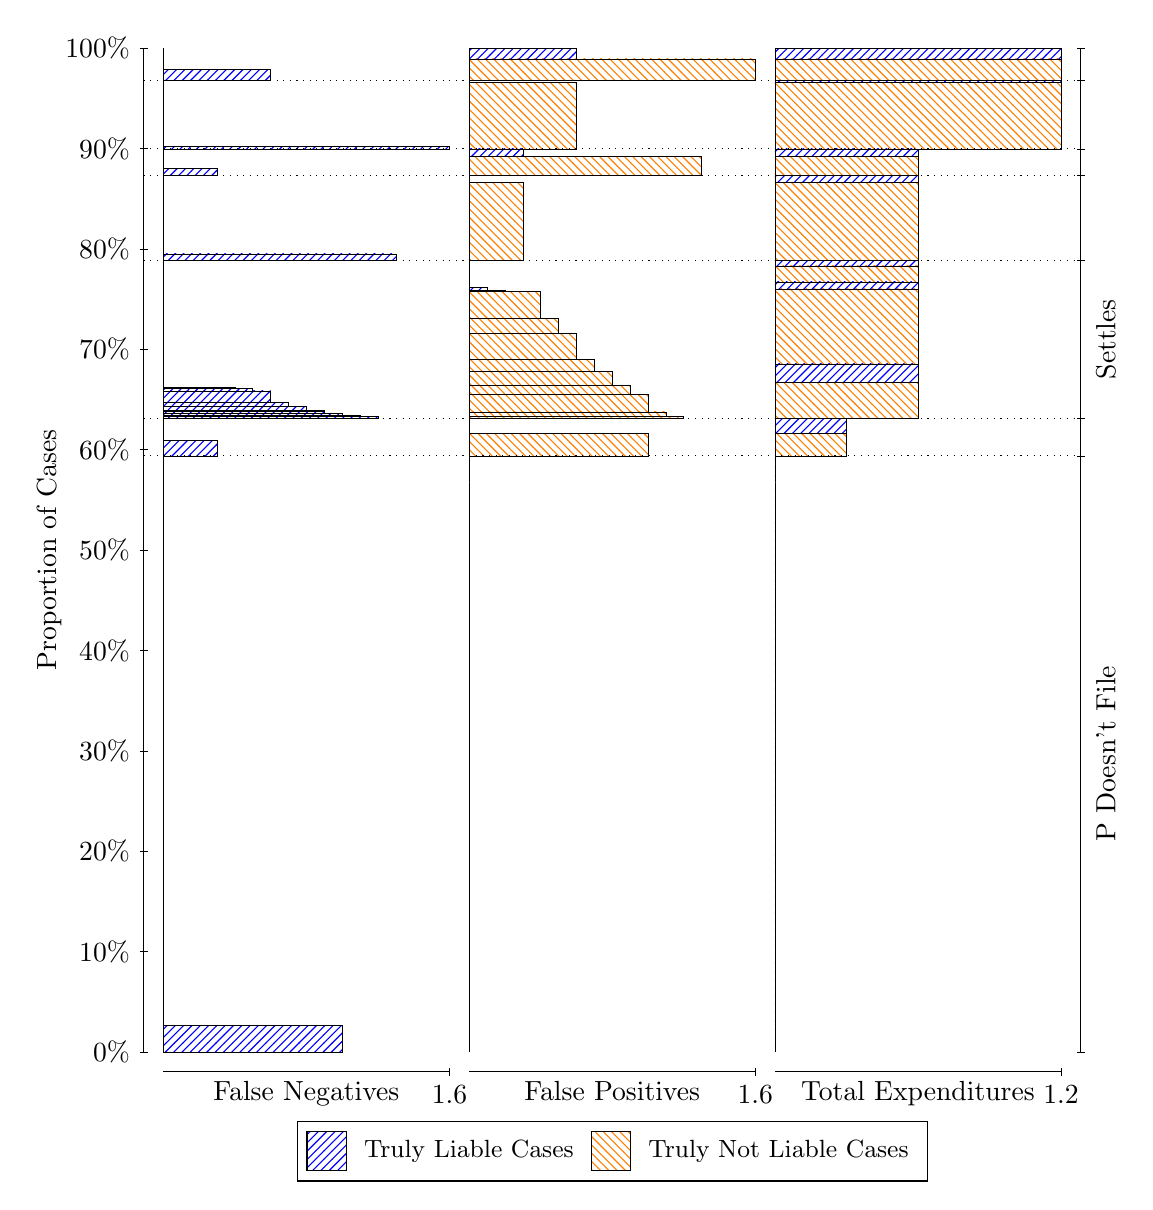
\begin{tikzpicture}
\draw[black, very thin] (1.5,1.75) -- (1.5,14.5);
\node[rotate=90, anchor=center] at (0.3, 8.125) {Proportion of Cases};
\draw[black, very thin] (1.45,1.75) -- (1.55,1.75);
\node[anchor=east] at (1.45, 1.75) {0\%};
\draw[black, very thin] (1.45,3.025) -- (1.55,3.025);
\node[anchor=east] at (1.45, 3.025) {10\%};
\draw[black, very thin] (1.45,4.3) -- (1.55,4.3);
\node[anchor=east] at (1.45, 4.3) {20\%};
\draw[black, very thin] (1.45,5.575) -- (1.55,5.575);
\node[anchor=east] at (1.45, 5.575) {30\%};
\draw[black, very thin] (1.45,6.85) -- (1.55,6.85);
\node[anchor=east] at (1.45, 6.85) {40\%};
\draw[black, very thin] (1.45,8.125) -- (1.55,8.125);
\node[anchor=east] at (1.45, 8.125) {50\%};
\draw[black, very thin] (1.45,9.4) -- (1.55,9.4);
\node[anchor=east] at (1.45, 9.4) {60\%};
\draw[black, very thin] (1.45,10.675) -- (1.55,10.675);
\node[anchor=east] at (1.45, 10.675) {70\%};
\draw[black, very thin] (1.45,11.95) -- (1.55,11.95);
\node[anchor=east] at (1.45, 11.95) {80\%};
\draw[black, very thin] (1.45,13.225) -- (1.55,13.225);
\node[anchor=east] at (1.45, 13.225) {90\%};
\draw[black, very thin] (1.45,14.5) -- (1.55,14.5);
\node[anchor=east] at (1.45, 14.5) {100\%};

\draw[black, very thin] (13.4,1.75) -- (13.4,14.5);
\draw[black, very thin] (13.35,1.75) -- (13.45,1.75);
\node[anchor=west] at (13.35, 1.75) {};
\draw[black, very thin] (13.35,9.3211) -- (13.45,9.3211);
\node[anchor=west] at (13.35, 9.3211) {};
\draw[black, very thin] (13.35,9.8005) -- (13.45,9.8005);
\node[anchor=west] at (13.35, 9.8005) {};
\draw[black, very thin] (13.35,11.804) -- (13.45,11.804);
\node[anchor=west] at (13.35, 11.804) {};
\draw[black, very thin] (13.35,12.878) -- (13.45,12.878);
\node[anchor=west] at (13.35, 12.878) {};
\draw[black, very thin] (13.35,13.219) -- (13.45,13.219);
\node[anchor=west] at (13.35, 13.219) {};
\draw[black, very thin] (13.35,14.093) -- (13.45,14.093);
\node[anchor=west] at (13.35, 14.093) {};
\draw[black, very thin] (13.35,14.5) -- (13.45,14.5);
\node[anchor=west] at (13.35, 14.5) {};

\draw[black, very thin, pattern color=blue, pattern=north east lines] (1.75,1.75) rectangle (4.0208,2.0914);
\draw[black, very thin, pattern color=orange, pattern=north west lines] (1.75,2.0914) rectangle (1.75,9.3211);
\draw[black, very thin, pattern color=blue, pattern=north east lines] (1.75,9.3211) rectangle (2.4312,9.5143);
\draw[black, very thin, pattern color=orange, pattern=north west lines] (1.75,9.5143) rectangle (1.75,9.8005);
\draw[black, very thin, pattern color=blue, pattern=north east lines] (1.75,9.8005) rectangle (4.475,9.8178);
\draw[black, very thin, pattern color=blue, pattern=north east lines] (1.75,9.8178) rectangle (4.2479,9.8326);
\draw[black, very thin, pattern color=blue, pattern=north east lines] (1.75,9.8326) rectangle (4.0208,9.8607);
\draw[black, very thin, pattern color=blue, pattern=north east lines] (1.75,9.8607) rectangle (3.7937,9.8883);
\draw[black, very thin, pattern color=blue, pattern=north east lines] (1.75,9.8883) rectangle (3.7937,9.9002);
\draw[black, very thin, pattern color=blue, pattern=north east lines] (1.75,9.9002) rectangle (3.5667,9.9503);
\draw[black, very thin, pattern color=blue, pattern=north east lines] (1.75,9.9503) rectangle (3.3396,9.9958);
\draw[black, very thin, pattern color=blue, pattern=north east lines] (1.75,9.9958) rectangle (3.1125,10.146);
\draw[black, very thin, pattern color=blue, pattern=north east lines] (1.75,10.146) rectangle (2.8854,10.18);
\draw[black, very thin, pattern color=blue, pattern=north east lines] (1.75,10.18) rectangle (2.6583,10.193);
\draw[black, very thin, pattern color=orange, pattern=north west lines] (1.75,10.193) rectangle (1.75,11.804);
\draw[black, very thin, pattern color=blue, pattern=north east lines] (1.75,11.804) rectangle (4.7021,11.887);
\draw[black, very thin, pattern color=orange, pattern=north west lines] (1.75,11.887) rectangle (1.75,12.878);
\draw[black, very thin, pattern color=blue, pattern=north east lines] (1.75,12.878) rectangle (2.4312,12.975);
\draw[black, very thin, pattern color=orange, pattern=north west lines] (1.75,12.975) rectangle (1.75,13.219);
\draw[black, very thin, pattern color=blue, pattern=north east lines] (1.75,13.219) rectangle (5.3833,13.249);
\draw[black, very thin, pattern color=orange, pattern=north west lines] (1.75,13.249) rectangle (1.75,14.093);
\draw[black, very thin, pattern color=blue, pattern=north east lines] (1.75,14.093) rectangle (3.1125,14.231);
\draw[black, very thin, pattern color=orange, pattern=north west lines] (1.75,14.231) rectangle (1.75,14.5);
\draw[black, very thin, pattern color=orange, pattern=north west lines] (5.6333,1.75) rectangle (5.6333,8.9797);
\draw[black, very thin, pattern color=blue, pattern=north east lines] (5.6333,8.9797) rectangle (5.6333,9.3211);
\draw[black, very thin, pattern color=orange, pattern=north west lines] (5.6333,9.3211) rectangle (7.9042,9.6074);
\draw[black, very thin, pattern color=blue, pattern=north east lines] (5.6333,9.6074) rectangle (5.6333,9.8005);
\draw[black, very thin, pattern color=orange, pattern=north west lines] (5.6333,9.8005) rectangle (8.3583,9.8254);
\draw[black, very thin, pattern color=orange, pattern=north west lines] (5.6333,9.8254) rectangle (8.1313,9.8788);
\draw[black, very thin, pattern color=orange, pattern=north west lines] (5.6333,9.8788) rectangle (7.9042,10.103);
\draw[black, very thin, pattern color=orange, pattern=north west lines] (5.6333,10.103) rectangle (7.6771,10.22);
\draw[black, very thin, pattern color=orange, pattern=north west lines] (5.6333,10.22) rectangle (7.45,10.396);
\draw[black, very thin, pattern color=orange, pattern=north west lines] (5.6333,10.396) rectangle (7.2229,10.543);
\draw[black, very thin, pattern color=orange, pattern=north west lines] (5.6333,10.543) rectangle (6.9958,10.875);
\draw[black, very thin, pattern color=orange, pattern=north west lines] (5.6333,10.875) rectangle (6.7687,11.066);
\draw[black, very thin, pattern color=orange, pattern=north west lines] (5.6333,11.066) rectangle (6.5417,11.411);
\draw[black, very thin, pattern color=blue, pattern=north east lines] (5.6333,11.411) rectangle (6.0875,11.424);
\draw[black, very thin, pattern color=blue, pattern=north east lines] (5.6333,11.424) rectangle (5.8604,11.458);
\draw[black, very thin, pattern color=blue, pattern=north east lines] (5.6333,11.458) rectangle (5.6333,11.804);
\draw[black, very thin, pattern color=orange, pattern=north west lines] (5.6333,11.804) rectangle (6.3146,12.795);
\draw[black, very thin, pattern color=blue, pattern=north east lines] (5.6333,12.795) rectangle (5.6333,12.878);
\draw[black, very thin, pattern color=orange, pattern=north west lines] (5.6333,12.878) rectangle (8.5854,13.122);
\draw[black, very thin, pattern color=blue, pattern=north east lines] (5.6333,13.122) rectangle (6.3146,13.219);
\draw[black, very thin, pattern color=orange, pattern=north west lines] (5.6333,13.219) rectangle (6.9958,14.063);
\draw[black, very thin, pattern color=blue, pattern=north east lines] (5.6333,14.063) rectangle (5.6333,14.093);
\draw[black, very thin, pattern color=orange, pattern=north west lines] (5.6333,14.093) rectangle (9.2667,14.362);
\draw[black, very thin, pattern color=blue, pattern=north east lines] (5.6333,14.362) rectangle (6.9958,14.5);
\draw[black, very thin, pattern color=orange, pattern=north west lines] (9.5167,1.75) rectangle (9.5167,8.9797);
\draw[black, very thin, pattern color=blue, pattern=north east lines] (9.5167,8.9797) rectangle (9.5167,9.3211);
\draw[black, very thin, pattern color=orange, pattern=north west lines] (9.5167,9.3211) rectangle (10.425,9.6074);
\draw[black, very thin, pattern color=blue, pattern=north east lines] (9.5167,9.6074) rectangle (10.425,9.8005);
\draw[black, very thin, pattern color=orange, pattern=north west lines] (9.5167,9.8005) rectangle (11.333,10.254);
\draw[black, very thin, pattern color=blue, pattern=north east lines] (9.5167,10.254) rectangle (11.333,10.489);
\draw[black, very thin, pattern color=orange, pattern=north west lines] (9.5167,10.489) rectangle (11.333,11.441);
\draw[black, very thin, pattern color=blue, pattern=north east lines] (9.5167,11.441) rectangle (11.333,11.529);
\draw[black, very thin, pattern color=orange, pattern=north west lines] (9.5167,11.529) rectangle (11.333,11.734);
\draw[black, very thin, pattern color=blue, pattern=north east lines] (9.5167,11.734) rectangle (11.333,11.804);
\draw[black, very thin, pattern color=orange, pattern=north west lines] (9.5167,11.804) rectangle (11.333,12.795);
\draw[black, very thin, pattern color=blue, pattern=north east lines] (9.5167,12.795) rectangle (11.333,12.878);
\draw[black, very thin, pattern color=orange, pattern=north west lines] (9.5167,12.878) rectangle (11.333,13.122);
\draw[black, very thin, pattern color=blue, pattern=north east lines] (9.5167,13.122) rectangle (11.333,13.219);
\draw[black, very thin, pattern color=orange, pattern=north west lines] (9.5167,13.219) rectangle (13.15,14.063);
\draw[black, very thin, pattern color=blue, pattern=north east lines] (9.5167,14.063) rectangle (13.15,14.093);
\draw[black, very thin, pattern color=orange, pattern=north west lines] (9.5167,14.093) rectangle (13.15,14.362);
\draw[black, very thin, pattern color=blue, pattern=north east lines] (9.5167,14.362) rectangle (13.15,14.5);
\draw[black, dotted] (1.5,9.3211) -- (13.4,9.3211);
\draw[black, dotted] (1.5,9.8005) -- (13.4,9.8005);
\draw[black, dotted] (1.5,11.804) -- (13.4,11.804);
\draw[black, dotted] (1.5,12.878) -- (13.4,12.878);
\draw[black, dotted] (1.5,13.219) -- (13.4,13.219);
\draw[black, dotted] (1.5,14.093) -- (13.4,14.093);
\draw[black, very thin] (1.75,1.5) -- (5.3833,1.5);
\node[anchor=north] at (3.5667, 1.5) {False Negatives};
\draw[black, very thin] (5.3833,1.45) -- (5.3833,1.55);
\node[anchor=north] at (5.3833, 1.45) {1.6};

\draw[black, very thin] (5.6333,1.5) -- (9.2667,1.5);
\node[anchor=north] at (7.45, 1.5) {False Positives};
\draw[black, very thin] (9.2667,1.45) -- (9.2667,1.55);
\node[anchor=north] at (9.2667, 1.45) {1.6};

\draw[black, very thin] (9.5167,1.5) -- (13.15,1.5);
\node[anchor=north] at (11.333, 1.5) {Total Expenditures};
\draw[black, very thin] (13.15,1.45) -- (13.15,1.55);
\node[anchor=north] at (13.15, 1.45) {1.2};

\node[black, centered, rotate=90] at (13.72, 5.5356) {P Doesn't File};

\node[black, centered, rotate=90] at (13.72, 10.802) {Settles};





\draw (7.449999999999999,1.5) node[draw=none] (baseCoordinate) {};
\begin{scope}[align=center]
        \matrix[scale=0.5, draw=black, below=0.5cm of baseCoordinate, nodes={draw}, column sep=0.1cm]{
            \node[rectangle, draw, minimum width=0.5cm, minimum height=0.5cm, pattern=north east lines, pattern color=blue] {}; &
            \node[draw=none, font=\small] (B) {Truly Liable Cases}; &
            \node[rectangle, draw, minimum width=0.5cm, minimum height=0.5cm, pattern=north west lines, pattern color=orange] {}; &
            \node[draw=none, font=\small] (B) {Truly Not Liable Cases}; \\
            };
\end{scope}

\end{tikzpicture}
\end{document}